\chapter{酸、碱与 pH}\label{ch:g9:acids-bases-ph}

厨房的架子上放着一个柠檬、一瓶醋、一块肥皂和一盒小苏打；
水槽下面放着一瓶管道疏通剂，瓶身贴着黑红两色的警示标签。
这些东西中，有的尝起来发酸，有的摸上去滑溜，
有的还会灼伤皮肤。一把编号从 0 到 14 的标尺，就能将它们全部分类——
同一把标尺，还用于测量游泳池、花园土壤、
血液和海洋。

\begin{recall}
\omterm{def:g9:ions:ion}{离子}是带电荷的\omterm{def:g7:atoms-and-molecules:atom}{原子}或\omterm{def:g7:atoms-and-molecules:atom}{原子}团；\omterm{def:g9:ions:ion}{阳离子}如 \ce{Na+} 带正电，
\omterm{def:g9:ions:ion}{阴离子}如 \ce{Cl-} 或 \ce{OH-} 带负电。
\omterm{def:g9:ions:ion}{离子}溶液中含有标注 (aq) 的\omterm{def:g9:ions:ion}{离子}，这些\omterm{def:g9:ions:ion}{离子}能自由移动
（见\cref{ch:g9:ions}）。
\end{recall}

\begin{omfigure}
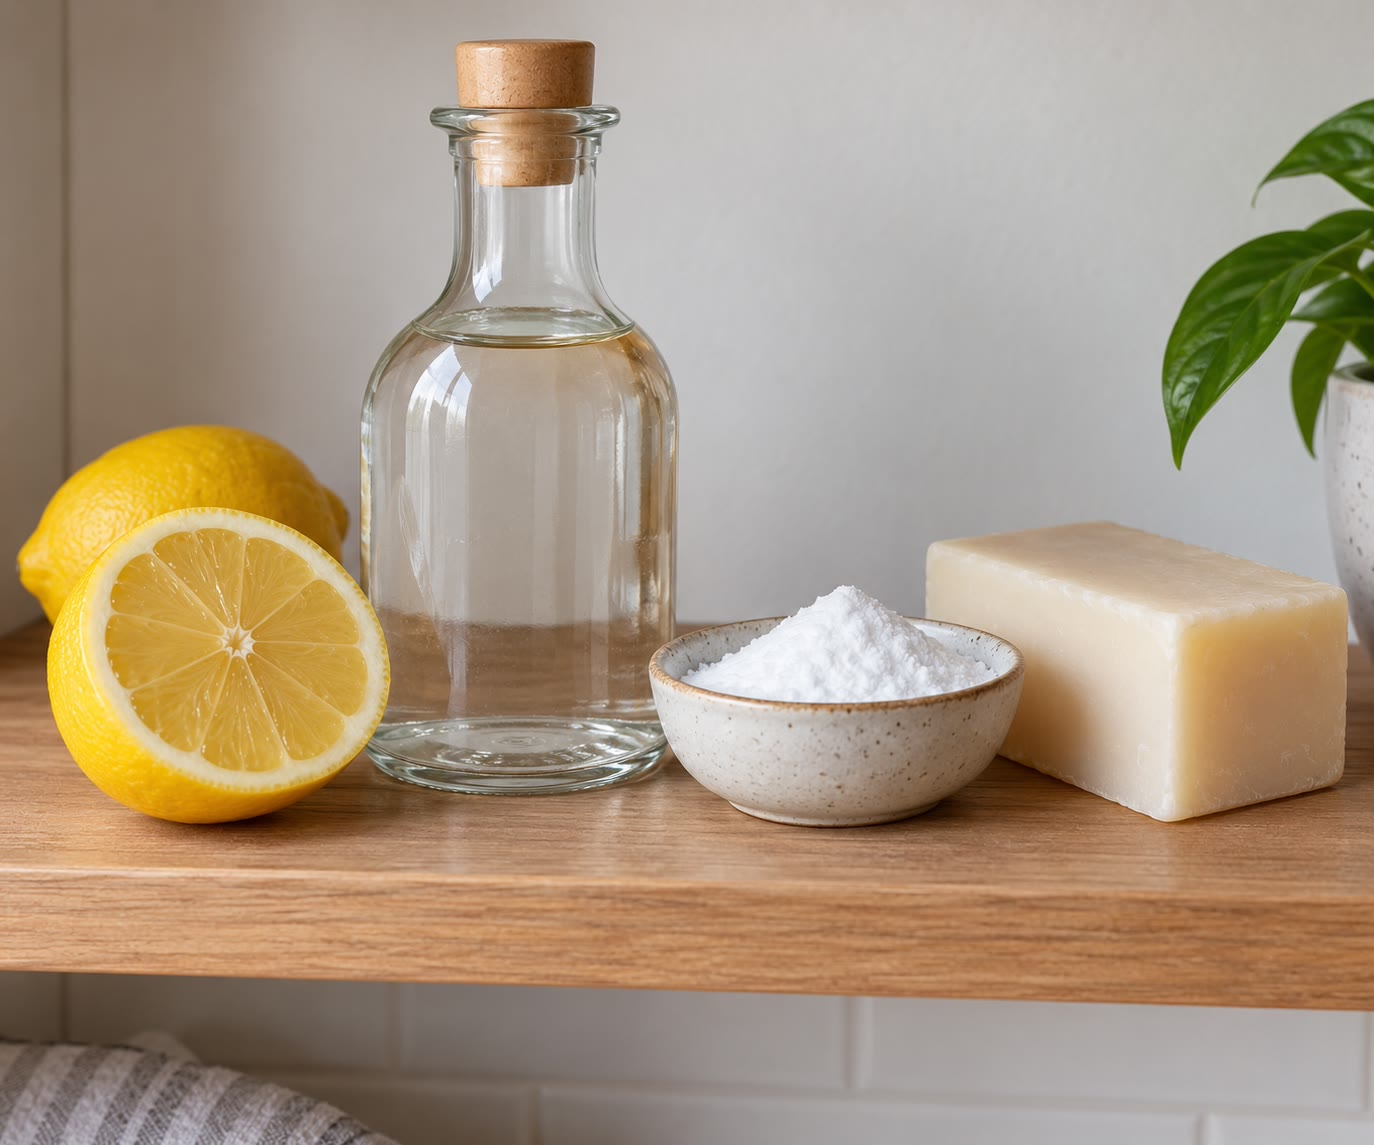
\includegraphics[width=0.55\linewidth]{images/book1/ai/g9-kitchen-shelf.jpg}

{\small 柠檬、醋、肥皂和小苏打：厨房里的
酸和碱。}
\end{omfigure}

\section{酸性、碱性和中性溶液}

\begin{definition}[酸性、碱性和中性溶液]\label{def:g9:acids-bases-ph:acidic}
任何\omterm{def:g6:solutions-and-solubility:solute}{水溶液}中都含有氢\omterm{def:g9:ions:ion}{离子} \ce{H+(aq)}
和氢氧根\omterm{def:g9:ions:ion}{离子} \ce{OH-(aq)}。
若溶液中 \ce{H+} \omterm{def:g9:ions:ion}{离子}比 \ce{OH-} \omterm{def:g9:ions:ion}{离子}多，则称为
\emph{酸性溶液}\index{酸性溶液}；若 \ce{OH-} \omterm{def:g9:ions:ion}{离子}比 \ce{H+} \omterm{def:g9:ions:ion}{离子}多，
则称为\emph{碱性溶液}\index{碱性溶液}；若两种\omterm{def:g9:ions:ion}{离子}数目相等，
则称为\emph{中性溶液}\index{中性溶液}。
\end{definition}

\begin{example}[三种溶液]\label{ex:g9:acids-bases-ph:three}
盐酸是\omterm{def:g9:acids-bases-ph:acidic}{酸性溶液}，其中含有 \ce{H+(aq)} 和 \ce{Cl-(aq)} \omterm{def:g9:ions:ion}{离子}，
\ce{OH-} \omterm{def:g9:ions:ion}{离子}则极少。氢氧化钠溶液是\omterm{def:g9:acids-bases-ph:acidic}{碱性溶液}，
含有 \ce{Na+(aq)} 和 \ce{OH-(aq)} \omterm{def:g9:ions:ion}{离子}，而 \ce{H+} \omterm{def:g9:ions:ion}{离子}极少。
纯水和盐水都是中性的。
\end{example}

\section{pH 标度}

\begin{definition}[pH]\label{def:g9:acids-bases-ph:ph}
\omterm{def:g6:solutions-and-solubility:solute}{水溶液}的 \emph{pH}\index{pH} 是一个数，通常在 0 到 14 之间，
用来表示溶液的酸碱程度：在 \qty{25}{\celsius} 时，\omterm{def:g9:acids-bases-ph:acidic}{中性溶液}的 pH 为 7，
\omterm{def:g9:acids-bases-ph:acidic}{酸性溶液}的 pH 低于 7，\omterm{def:g9:acids-bases-ph:acidic}{碱性溶液}的 pH 高于 7。
溶液所含的 \ce{H+} \omterm{def:g9:ions:ion}{离子}越多，
其 pH 就越低。
\end{definition}

\begin{omfigure}
\begin{tikzpicture}[font=\small, x=0.95cm]
  \foreach \k in {0,...,13} {
    \pgfmathtruncatemacro\rr{2.2*max(0,100-14.3*\k)+30}
    \pgfmathtruncatemacro\gg{1.8*(\k<7 ? 30+10*\k : 100-8*(\k-7))+40}
    \pgfmathtruncatemacro\bb{2.2*max(0,14.3*(\k-6))+30}
    \definecolor{phc}{RGB}{\rr,\gg,\bb}
    \fill[phc] (\k,0) rectangle ++(1,0.6);
  }
  \foreach \k in {0,...,14} \node[anchor=north, font=\footnotesize] at (\k,-0.02) {\k};
  \draw[black!60] (0,0) rectangle (14,0.6);
  \node[anchor=south] at (3.5,0.65) {酸性};
  \node[anchor=south] at (7,0.65) {中性};
  \node[anchor=south] at (10.5,0.65) {碱性};
  % ledger: ph:HCl-1M, ph:gastric, ph:lime, ph:wine, ph:coffee, ph:pure-water, ph:seawater, ph:milk-magnesia, ph:ammonia, ph:NaOH-1M
  \foreach \x/\lab/\lev/\anc in {0/{盐酸 \\（1 M）}/1/north, 1.5/{胃液}/3/north east,
      2/{青柠汁}/2/north west, 3.5/{葡萄酒}/1/north, 5/{咖啡}/2/north, 7/{纯水}/3/north,
      8.1/{海水}/1/north, 10.5/{氧化镁 \\乳}/3/north, 12/{家用 \\氨水}/1/north,
      14/{氢氧化钠 \\（1 M）}/2/north east} {
    \draw[black!55] (\x,-0.45) -- (\x,-0.45-0.8*\lev);
    \node[anchor=\anc, font=\footnotesize, align=center, inner sep=2pt] at (\x,-0.45-0.8*\lev) {\lab};
  }
\end{tikzpicture}

{\small \omterm{def:g9:acids-bases-ph:ph}{pH} 标度，以及一些常见溶液的 \omterm{def:g9:acids-bases-ph:ph}{pH}。}
\end{omfigure}

\begin{definition}[pH 试纸和 pH 计]\label{def:g9:acids-bases-ph:ph-paper}
\emph{pH 试纸}\index{pH 试纸}是一条浸有\omterm{def:g2:mixing-and-dissolving:mix}{混合}染料的纸，
在不同 \omterm{def:g9:acids-bases-ph:ph}{pH} 下呈现不同颜色；将一滴溶液滴在试纸上，
再把颜色与盒上印着的比色卡对照。
\emph{pH 计}\index{pH 计}用插入溶液中的玻璃探头测量 \omterm{def:g9:acids-bases-ph:ph}{pH}，
以数字形式显示结果，
可精确到小数点后一位或两位。
\end{definition}

\begin{method}[用 pH 试纸测量 pH]\label{met:g9:acids-bases-ph:paper}
\begin{enumerate}
  \item 取一小条 \omterm{def:g9:acids-bases-ph:ph}{pH} 试纸放在干净、干燥的表面皿上。
  \item 用干净的玻璃棒将一滴溶液
        点在试纸上（切勿把试纸浸入\omterm{def:g7:identifying-substances:characteristic-test}{试剂}瓶中）。
  \item 立即将颜色与比色卡对照，读出
        \omterm{def:g9:acids-bases-ph:ph}{pH}，通常精确到最接近的整数。
\end{enumerate}
\end{method}

\begin{omfigure}
\begin{tikzpicture}[font=\small, scale=1.2]
  \pic[transform shape] at (0,0) {stirrer};
  \pic[transform shape] at (0,0.05) {beaker={0.55}{omWater!80}};
  \pic[transform shape] at (0.25,0.35) {probe};
  \pic[transform shape] at (2.6,3.4) {meter={pH}};
  \draw[black!70, line width=0.6pt] (0.25,3.45) .. controls (0.3,4.3) and (2.2,4.4)
    .. (2.2,2.95);
  \draw[<-, omProp, thick] (0.4,1.0) -- (2.0,1.3) node[right, text=black] {玻璃探头};
  \draw[<-, omProp, thick] (3.35,3.4) -- (4.0,3.4) node[right, text=black] {pH 计};
  \draw[<-, omProp, thick] (-0.6,0.6) -- (-1.6,0.9) node[left, text=black] {溶液};
\end{tikzpicture}

{\small 用 \omterm{def:g9:acids-bases-ph:ph}{pH} 计测量 \omterm{def:g9:acids-bases-ph:ph}{pH}：玻璃探头浸入
溶液中，溶液被轻轻搅拌。}
\end{omfigure}

\section{稀释酸}

\begin{proposition}[稀释使 pH 趋近于 7]\label{prop:g9:acids-bases-ph:dilution}
向\omterm{def:g9:acids-bases-ph:acidic}{酸性溶液}中加水，会使其中的 \ce{H+} \omterm{def:g9:ions:ion}{离子}分散到更大的
体积中：\omterm{def:g9:acids-bases-ph:ph}{pH} 升高，趋近于 7，但不会超过 7。对于像
盐酸这样的酸，稀释十倍后 \omterm{def:g9:acids-bases-ph:ph}{pH} 约升高
一个单位：1 体积 \omterm{def:g9:acids-bases-ph:ph}{pH} 为 2 的酸与 9 体积的水\omterm{def:g2:mixing-and-dissolving:mix}{混合}，得到一种
\omterm{def:g9:acids-bases-ph:ph}{pH} 为 3 的溶液。稀释\omterm{def:g9:acids-bases-ph:acidic}{碱性溶液}同样会使其 \omterm{def:g9:acids-bases-ph:ph}{pH} 降低，
趋近于 7。
\end{proposition}

\begin{omfigure}
\begin{tikzpicture}[font=\small, scale=1.05]
  \foreach \k/\ph/\cc in {0/2/red!38!omWater,1/3/red!24!omWater,2/4/red!12!omWater} {
    \pic[transform shape] at (\k*4.4,0) {beaker={0.55}{\cc}};
    \node[anchor=north, align=center] at (\k*4.4,-0.15) {pH \ph};
  }
  \foreach \k in {0,1} \draw[->, thick, omProp] (\k*4.4+1.1,1.0) -- (\k*4.4+3.3,1.0)
    node[midway, above, text=black, font=\footnotesize, align=center]
    {10 mL + 90 mL\\ 水};
\end{tikzpicture}

{\small 将酸稀释十倍，再稀释十倍：\omterm{def:g9:acids-bases-ph:ph}{pH} 由
2 变为 3，再变为 4（每个烧杯中的溶液，都是取前一杯溶液的十分之一，
再加水稀释而成）。}
\end{omfigure}

\begin{inthelab}[稀释酸]
稀释酸时，老师总是把酸缓慢地倒入
水中，绝不能把水倒入酸中：\omterm{def:g2:mixing-and-dissolving:mix}{混合}时会放出热量，
若将水倒在浓酸上，水会立即沸腾，并把酸
溅出容器外。
\end{inthelab}

\section{生活中的酸和碱}

\begin{proposition}[身边的酸和碱]\label{prop:g9:acids-bases-ph:everyday}
酸性的有：柠檬汁和青柠汁、醋、葡萄酒、碳酸饮料、咖啡，
胃液。碱性的有：海水（略呈碱性）、小苏打
溶于水中、肥皂、氢氧化镁乳剂（一种治疗胃酸过多的药物）、
家用氨水、漂白剂、管道疏通剂（碱性很强）。
\end{proposition}

\begin{example}[海洋的 pH]\label{ex:g9:acids-bases-ph:ocean}
% ledger: ph:seawater, ph:ocean-drop
海洋的平均 \omterm{def:g9:acids-bases-ph:ph}{pH} 约为 8.1，略呈碱性。自
工业时代开始，\omterm{def:g2:mixing-and-dissolving:dissolve}{溶解}于\omterm{def:g4:air-a-mixture-of-gases:air}{空气}中的二氧化碳已使
表层海水的 \omterm{def:g9:acids-bases-ph:ph}{pH} 降低约 0.1：海洋正逐渐变得
碱性减弱，这对贝类和珊瑚有害。
\end{example}

\begin{omfigure}
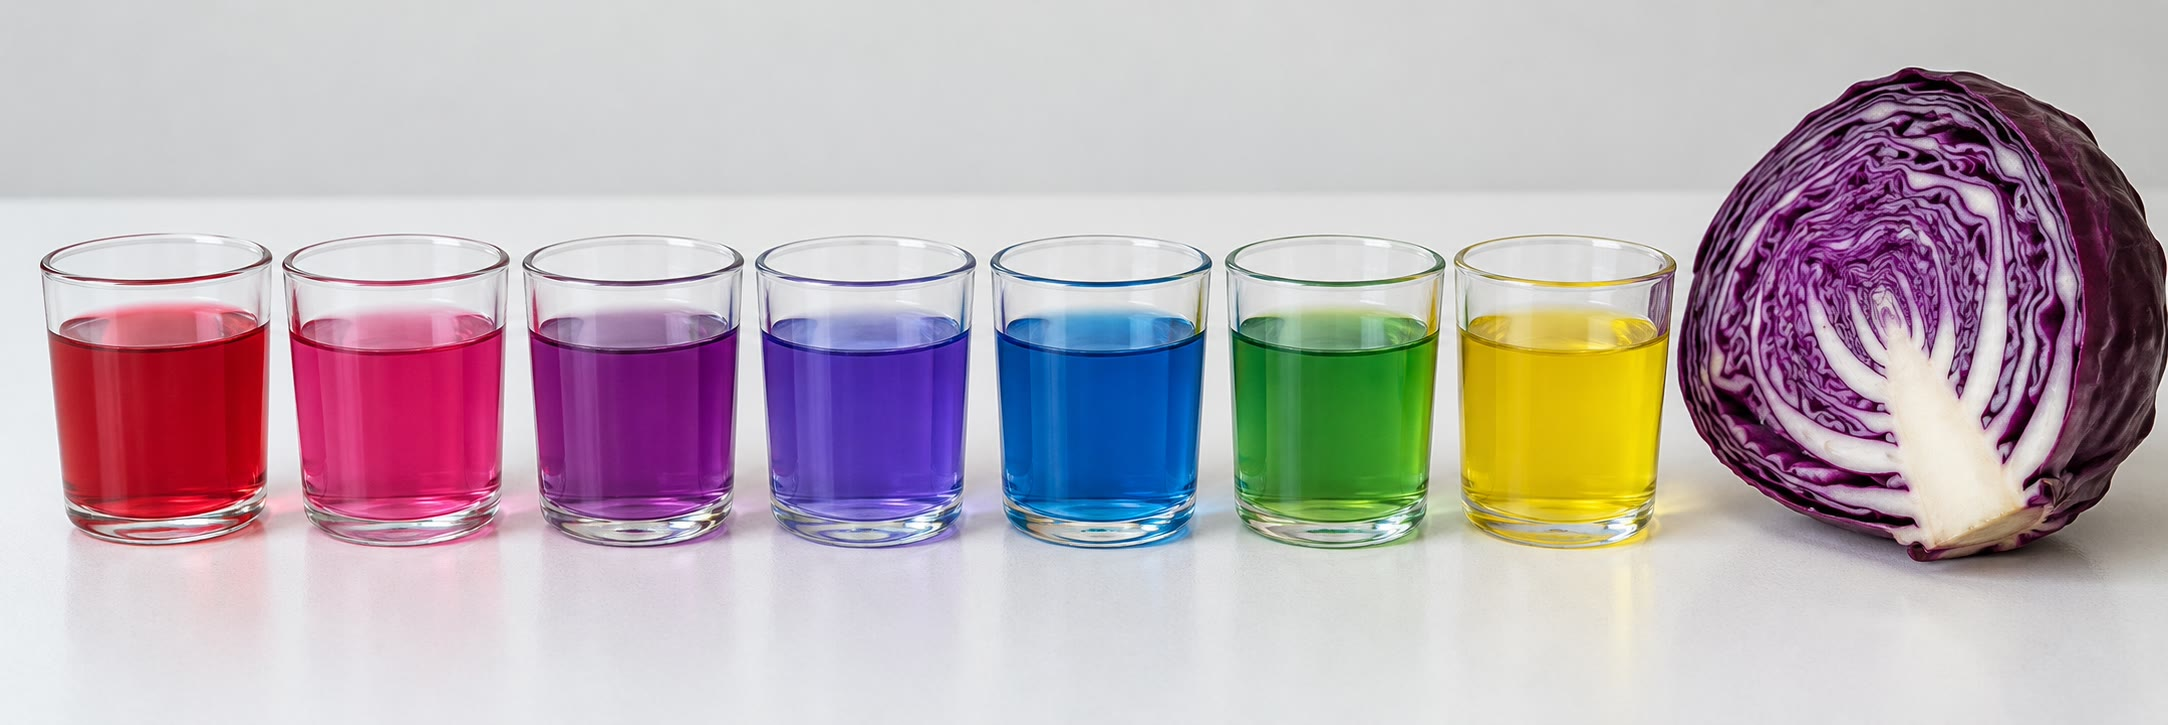
\includegraphics[width=0.55\linewidth]{images/book1/ai/g9-red-cabbage.jpg}

{\small 老师制备的紫甘蓝汁会随
\omterm{def:g9:acids-bases-ph:ph}{pH} 变化颜色：酸性中呈红色，接近中性时呈紫色，随碱性增强依次为蓝色、绿色，
再到碱性越来越强的溶液中呈黄色。}
\end{omfigure}

\section{腐蚀性产品的安全}

\begin{safety}{\ghs[0.85cm]{GHS05}\ghs[0.85cm]{GHS07}}
% ledger: ghs:HCl, ghs:NaOH
浓盐酸与氢氧化钠（管道疏通剂中的
碱）带有腐蚀性象形图 GHS05：会对
皮肤和眼睛造成严重灼伤，并腐蚀金属。GHS07：刺激性。戴护目镜和手套；
一旦溅到，应立即用大量清水冲洗。
\end{safety}

\begin{remark}[切勿混用清洁用品]\label{rem:g9:acids-bases-ph:mix}
酸性产品与碱性产品会相互反应，有时反应十分剧烈，有些
\omterm{def:g6:pure-substances-and-mixtures:mixture}{混合物}会释放有毒气体：漂白剂与酸性除垢剂\omterm{def:g2:mixing-and-dissolving:mix}{混合}会
释放氯气。清洁用品绝不能混用。
\end{remark}

\section{练习}

\begin{exercise}[$\star$]\label{exo:g9:acids-bases-ph:1}
判断下列溶液是酸性、碱性还是中性：\omterm{def:g9:acids-bases-ph:ph}{pH} 为 3 的溶液、\omterm{def:g9:acids-bases-ph:ph}{pH} 为 7 的
溶液、\omterm{def:g9:acids-bases-ph:ph}{pH} 为 11 的溶液。
\end{exercise}

\begin{exercise}[$\star$]\label{exo:g9:acids-bases-ph:2}
\omterm{def:g9:acids-bases-ph:acidic}{酸性溶液}中哪种\omterm{def:g9:ions:ion}{离子}的数目更多？\omterm{def:g9:acids-bases-ph:acidic}{碱性溶液}中呢？
\end{exercise}

\begin{exercise}[$\star$]\label{exo:g9:acids-bases-ph:3}
利用本章的 \omterm{def:g9:acids-bases-ph:ph}{pH} 标尺，把下列物质按从最酸到
最碱的顺序排列：咖啡、海水、青柠汁、家用氨水、
纯水。
\end{exercise}

\begin{exercise}[$\star$]\label{exo:g9:acids-bases-ph:4}
说明如何用 \omterm{def:g9:acids-bases-ph:ph}{pH} 试纸测定溶液的 \omterm{def:g9:acids-bases-ph:ph}{pH}。
\end{exercise}

\begin{exercise}[$\star\star$]\label{exo:g9:acids-bases-ph:5}
将 \omterm{def:g9:acids-bases-ph:ph}{pH} 为 4 的溶液用水稀释十倍，稀释后的 \omterm{def:g9:acids-bases-ph:ph}{pH}
约为多少？若稀释一百倍，又是多少？
\end{exercise}

\begin{exercise}[$\star\star$]\label{exo:g9:acids-bases-ph:6}
向\omterm{def:g9:acids-bases-ph:acidic}{酸性溶液}中加水，能否使其变为碱性？请说明理由。
\end{exercise}

\begin{exercise}[$\star\star$]\label{exo:g9:acids-bases-ph:7}
为什么稀释酸时必须把酸倒入水中，而不能反过来？
\end{exercise}

\begin{exercise}[$\star\star$]\label{exo:g9:acids-bases-ph:8}
一瓶\omterm{def:g7:identifying-substances:characteristic-test}{试剂}带有 GHS05 图标。它表示什么含义？给出两条
防范措施。
\end{exercise}

\begin{exercise}[$\star\star$]\label{exo:g9:acids-bases-ph:9}
要使某酸的 \omterm{def:g9:acids-bases-ph:ph}{pH} 由 1 变为
4，需要进行几次十倍稀释？总稀释倍数为多少？
\end{exercise}

\begin{exercise}[$\star\star$]\label{exo:g9:acids-bases-ph:10}
氢氧化镁乳剂用于缓解胃酸过多。利用 \omterm{def:g9:acids-bases-ph:ph}{pH} 标度，
试解释其原因。
\end{exercise}

\begin{exercise}[$\star\star\star$]\label{exo:g9:acids-bases-ph:11}
自工业时代以来，海洋的 \omterm{def:g9:acids-bases-ph:ph}{pH} 约下降了 0.1。今天的海洋
是否呈酸性？其变化趋势如何，原因是什么？
\end{exercise}

\begin{exercise}[$\star\star\star$]\label{exo:g9:acids-bases-ph:12}
某同学用 \omterm{def:g9:acids-bases-ph:ph}{pH} 试纸测得该食醋的 \omterm{def:g9:acids-bases-ph:ph}{pH} 为 3，
用 \omterm{def:g9:acids-bases-ph:ph}{pH} 计测得为 2.6。试解释两次结果不同的原因，
并说明哪种方法更精确。
\end{exercise}

\section{问题：酸液泄漏}

\begin{problem}[{周末问题——一升酸液溅入实验室水槽，
以及为何稀释并非解决办法}]
\label{pb:g9:acids-bases-ph:1}
一瓶装有 \qty{1}{L} 的稀盐酸，\omterm{def:g9:acids-bases-ph:ph}{pH} 为 2，
在实验室水槽中摔碎。排水管不得接收
任何 \omterm{def:g9:acids-bases-ph:ph}{pH} 低于 5 的溶液。取本章规律：对于该酸，每稀释十倍，
\omterm{def:g9:acids-bases-ph:ph}{pH} 升高一个单位。

\medskip
\noindent\textbf{第一部分——酸液。}
\begin{enumerate}
  \item 该溶液呈酸性、中性还是碱性？它含量最多的
        是哪种\omterm{def:g9:ions:ion}{离子}？
  \item 该\omterm{def:g7:identifying-substances:characteristic-test}{试剂}瓶应贴哪种图标？为什么？
  \item 老师用 \omterm{def:g9:acids-bases-ph:ph}{pH} 计而不用 \omterm{def:g9:acids-bases-ph:ph}{pH} 试纸测定 \omterm{def:g9:acids-bases-ph:ph}{pH}。
        请说出一项优点。
  \item 同种酸中，\omterm{def:g9:acids-bases-ph:ph}{pH} 为 2 的一升溶液比
        \omterm{def:g9:acids-bases-ph:ph}{pH} 为 3 的一升溶液多出多少个 \ce{H+} \omterm{def:g9:ions:ion}{离子}？
\end{enumerate}

\medskip
\noindent\textbf{第二部分——稀释。}
\begin{enumerate}[resume]
  \item 将这一升酸稀释十倍后，所得溶液的
        体积为多少？其 \omterm{def:g9:acids-bases-ph:ph}{pH} 为多少？
  \item 要使 \omterm{def:g9:acids-bases-ph:ph}{pH} 达到 5，需要进行几次十倍稀释？
  \item 这样得到的溶液总体积为多少？
  \item 加入任意量的水，能否使溶液变为碱性？请说明。
\end{enumerate}

\medskip
\noindent\textbf{第三部分——更好的方法。}
老师改为逐滴加入碱溶液，直至
\omterm{def:g9:acids-bases-ph:ph}{pH} 试纸显示为 7：酸中的 \ce{H+} \omterm{def:g9:ions:ion}{离子}与
碱中的 \ce{OH-} \omterm{def:g9:ions:ion}{离子}发生反应。
\begin{enumerate}[resume]
  \item 写出 \ce{H+} 与 \ce{OH-}
        \omterm{def:g9:ions:ion}{离子}之间反应的方程式。
  \item 为什么这种方法比稀释更好？
  \item 举出一种日常生活中的碱性物质，可在厨房里用于
        清理少量溅出的食醋。
  \item 计算需向这一升酸中加入
        多少体积的水，才能使其 \omterm{def:g9:acids-bases-ph:ph}{pH} 变为 5。
\end{enumerate}
\end{problem}
